\documentclass{beamer}
\usepackage[english, russian]{babel}
\usepackage[T2A]{fontenc}
\usepackage[utf8]{inputenc}
\usepackage{indentfirst}
\usepackage{amsmath, amsfonts, amssymb, amsthm, mathtools}
\usepackage[export]{adjustbox}
\usepackage{graphicx} 
\graphicspath{ {./images/} }

\usepackage{subcaption}
\usepackage{verbatim}

\usepackage{minted}{\setlength{\parskip}{0pt}}

\usepackage{hyperref}

\hypersetup{
    colorlinks=true,
    linkcolor=blue,
    filecolor=magenta,      
    urlcolor=black,
    pdftitle={Overleaf Example},
    pdfpagemode=FullScreen,
    }


\title{Отчет по лабораторной работе № 9. \\Настройка POP3/IMAP сервера}
\author{Данила Стариков \\ НПИбд-02-22}
\date{2024}

\begin{document}
\maketitle
\newpage

\tableofcontents

\newpage
\section{Цель работы}
Приобретение практических навыков по установке и простейшему конфигурированию POP3/IMAP-сервера.
\newpage
\section{Выполнение работы}

\subsection{Установка Dovecot}
\begin{enumerate}
\item На виртуальной машине \texttt{server} вошли под пользователем и открыли терминал. Перешли в режим суперпользователя:
  \begin{minted}{bash}
    sudo -i
  \end{minted}
\item Установили необходимые для работы пакеты:
  \begin{minted}{bash}
    dnf -y install dovecot telnet
  \end{minted}
\end{enumerate}
\subsection{Настройка dovecot}
\begin{enumerate}
\item В конфигурационном файле \texttt{/etc/dovecot/dovecot.conf} прописали список почтовых протоколов, по которым разрешено работать Dovecot (Рис. \ref{01}):
  \begin{minted}{bash}
    protocols = imap pop3
  \end{minted}
\begin{center}
    \centering
    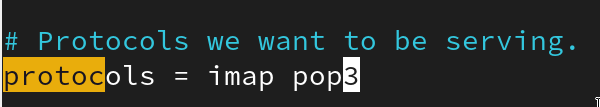
\includegraphics[width=\textwidth]{../images/image01.png}
    \captionof{figure}{Разрешенные почтовые протоколы в конфигурации Dovecot.}
    \label{01}
\end{center}

\item В конфигурационном файле \texttt{/etc/dovecot/conf.d/10-auth.conf} проверили, что указан метод аутентификации \texttt{plain} (Рис. \ref{02}):
\begin{minted}{bash}
  auth_mechanisms = plain
\end{minted}
\begin{center}
    \centering
    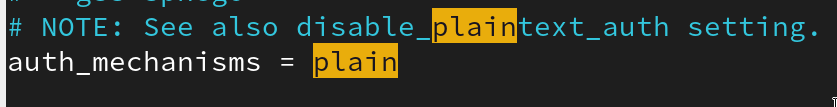
\includegraphics[width=\textwidth]{../images/image02.png}
    \captionof{figure}{Указание метода аутентификации \texttt{plain}.}
    \label{02}
\end{center}

\item В конфигурационном файле 
\texttt{/etc/dovecot/conf.d/auth-system.conf.ext} проверили, что для поиска пользователей и их паролей используется \texttt{pam} и файл \texttt{passwd} (Рис. \ref{03} и \ref{04}):
  \begin{minted}{bash}
    passdb {
      driver = pam
    }
    userdb {
      driver = passwd
    }
  \end{minted}
\begin{center}
    \centering
    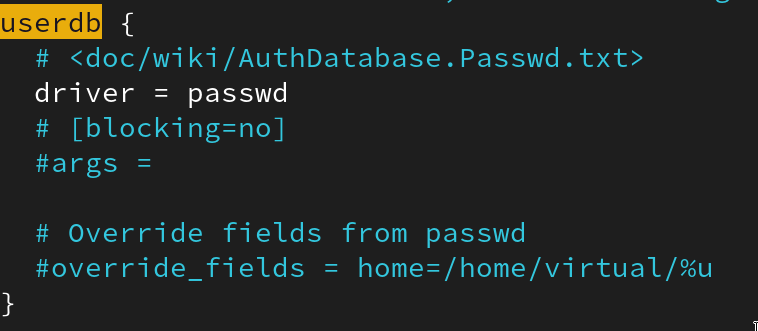
\includegraphics[width=\textwidth]{../images/image03.png}
    \captionof{figure}{Использование файла \texttt{passwd} для поиска паролей.}
    \label{03}
\end{center}
\begin{center}
    \centering
    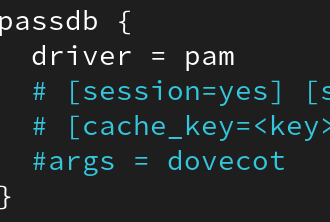
\includegraphics[width=\textwidth]{../images/image04.png}
    \captionof{figure}{Использование \texttt{pam} пользователей.}
    \label{04}
\end{center}

\item В конфигурационном файле \texttt{/etc/dovecot/conf.d/10-mail.conf} настроили месторасположение почтовых ящиков пользователей (Рис. \ref{05}):
  \begin{minted}{bash}
    mail_location = maildir:~/Maildir
  \end{minted}
\begin{center}
    \centering
    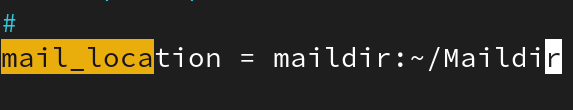
\includegraphics[width=\textwidth]{../images/image05.png}
    \captionof{figure}{Настройка месторасположения почтовых ящиков пользователей.}
    \label{05}
\end{center}

\item В Postfix задали каталог для доставки почты:
  \begin{minted}{bash}
    postconf -e 'home_mailbox = Maildir/'
  \end{minted}
\item Сконфигурировали межсетевой экран, разрешив работать службам протоколов POP3 и IMAP (Рис. \ref{06}):
  \begin{minted}{bash}
    firewall-cmd --get-services
    firewall-cmd --add-service=pop3 --permanent
    firewall-cmd --add-service=pop3s --permanent
    firewall-cmd --add-service=imap --permanent
    firewall-cmd --add-service=imaps --permanent
    firewall-cmd --reload
    firewall-cmd --list-services
  \end{minted}
\begin{center}
    \centering
    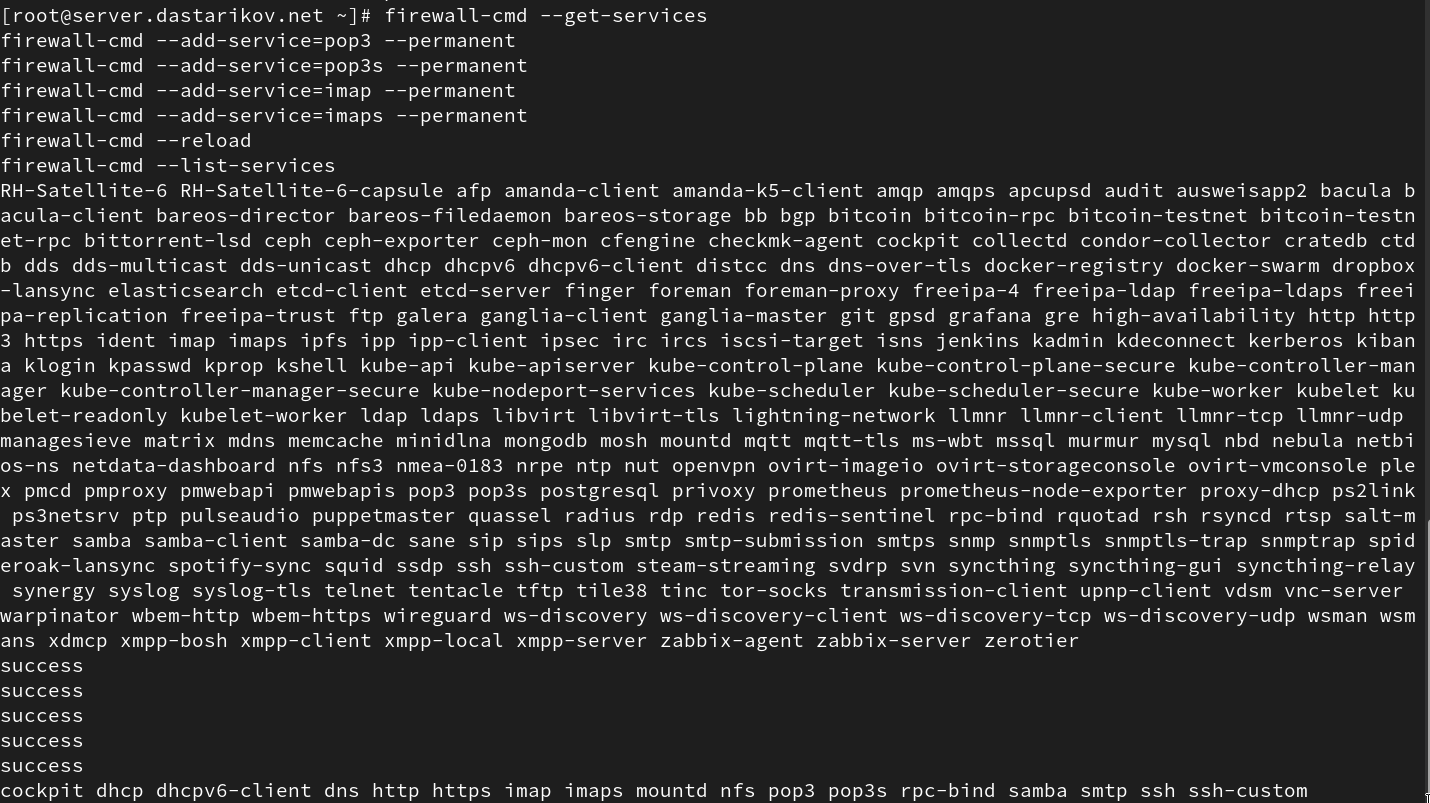
\includegraphics[width=\textwidth]{../images/image06.png}
    \captionof{figure}{Настройка межсетевого экрана для работы служб протоколов POP3 и IMAP.}
    \label{06}
\end{center}

\item Восстановили контекст безопасности в SELinux (Рис. \ref{07}):
  \begin{minted}{bash}
    restorecon -vR /etc
  \end{minted}
\begin{center}
    \centering
    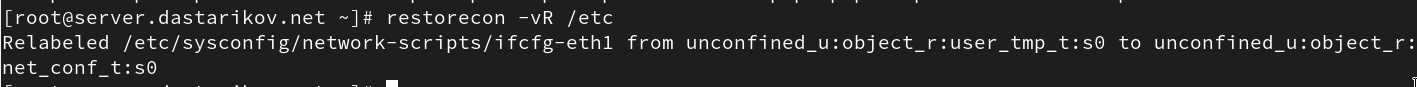
\includegraphics[width=\textwidth]{../images/image07.png}
    \captionof{figure}{Восстановление контекста безопасности в SELinux.}
    \label{07}
\end{center}

\item Перезапустили Postfix и запустили Dovecot (Рис. \ref{08}):
  \begin{minted}{bash}
    systemctl restart postfix
    systemctl enable dovecot
    systemctl start dovecot
  \end{minted}
\begin{center}
    \centering
    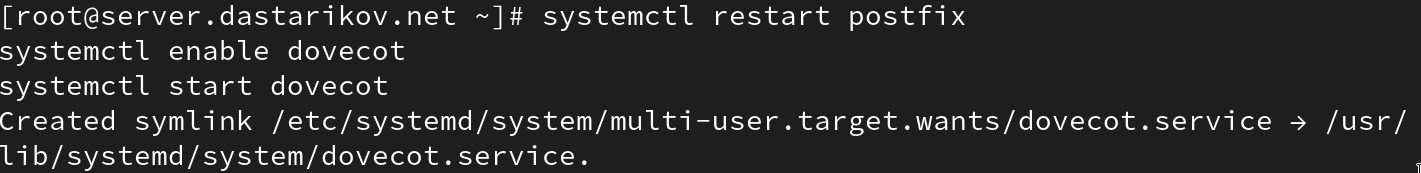
\includegraphics[width=\textwidth]{../images/image08.png}
    \captionof{figure}{Перезапуск Postfix и Dovecot.}
    \label{08}
\end{center}
\end{enumerate}


\subsection{Проверка работы Dovecot}
\begin{enumerate}
\item На дополнительном терминале виртуальной машины \texttt{server} запустили мониторинг работы почтовой службы (Рис. \ref{09}):
\begin{minted}{bash}
  tail -f /var/log/maillog
\end{minted}
\begin{center}
    \centering
    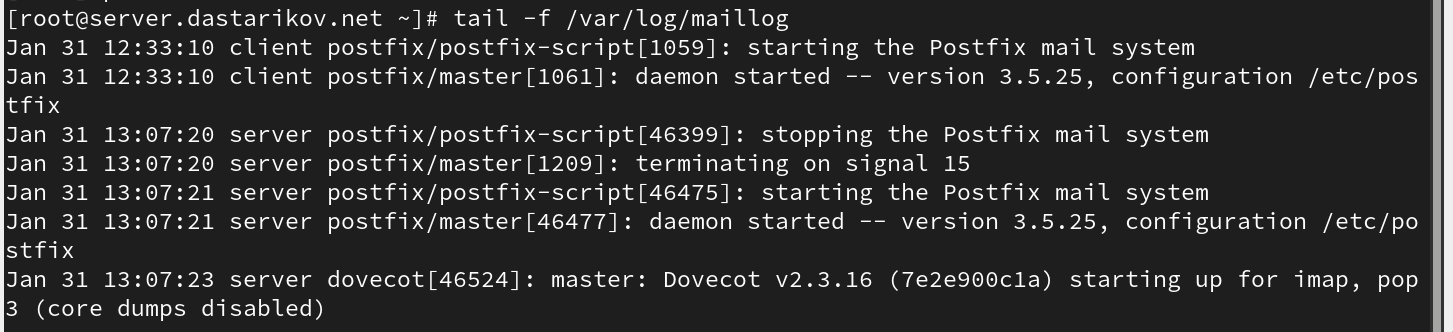
\includegraphics[width=\textwidth]{../images/image09.png}
    \captionof{figure}{Запуск мониторинга работы почтовой службы.}
    \label{09}
\end{center}

\item На терминале сервера для просмотра имеющейся почты использовали  (Рис. \ref{10})
  \begin{minted}{bash}
    MAIL=~/Maildir mail
  \end{minted}
\begin{center}
    \centering
    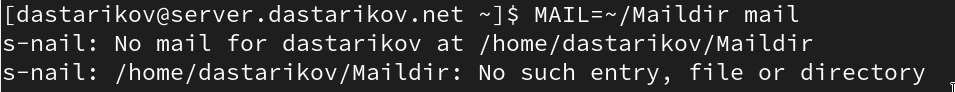
\includegraphics[width=\textwidth]{../images/image10.png}
    \captionof{figure}{Просмотр имеющейся почты на сервере.}
    \label{10}
\end{center}

\item Для просмотра \texttt{mailbox} пользователя на сервере на терминале с правами суперпользователя использовали команду (Рис. \ref{11})
  \begin{minted}{bash}
    doveadm mailbox list -u dastarikov
  \end{minted}
\begin{center}
    \centering
    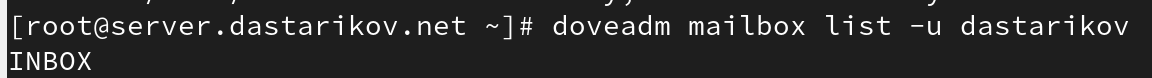
\includegraphics[width=\textwidth]{../images/image11.png}
    \captionof{figure}{Просмотр почты пользователя \texttt{dastarikov}.}
    \label{11}
\end{center}

\item На виртуальной машине \texttt{client} вошли под пользователем и открыли терминал. Перешли в режим суперпользователя:
  \begin{minted}{bash}
    sudo -i
  \end{minted}

\item Установили почтовый клиент:
  \begin{minted}{bash}
    dnf -y install evolution
  \end{minted}
\item Запустили и настроили почтовый клиент Evolution (Рис. \ref{12} и \ref{13}):
  \begin{itemize}
  \item в окне настройки учётной записи почты указали имя, адрес почты в виде \break \texttt{dastarikov@dastarikov.net}, ввели пароль пользователя, нажали <<Продолжить>>, затем нажали <<Настроить вручную>>;
  \item в качестве IMAP-сервера для входящих сообщений и SMTP-сервера для исходящих сообщений прописали \texttt{mail.dastarikov.net}, в качестве пользователя для входящих и исходящих сообщений указали \texttt{dastarikov};
  \item проверили номера портов: для IMAP — порт 143, для SMTP — порт 25;
  \item проверили настройки SSL и метода аутентификации: для IMAP — STARTTLS, аутентификация по обычному паролю, для SMTP — без аутентификации, аутентификация — <<Без аутентификации>>;
  \item при возникновении сообщения о небезопасном соединении выставили галочку о понимании риска работы по такому соединению и нажали <<Ок>>, затем подтвердили исключение безопасности, нажав в появившемся окне соответствующую кнопку.
\end{itemize}
\begin{center}
    \centering
    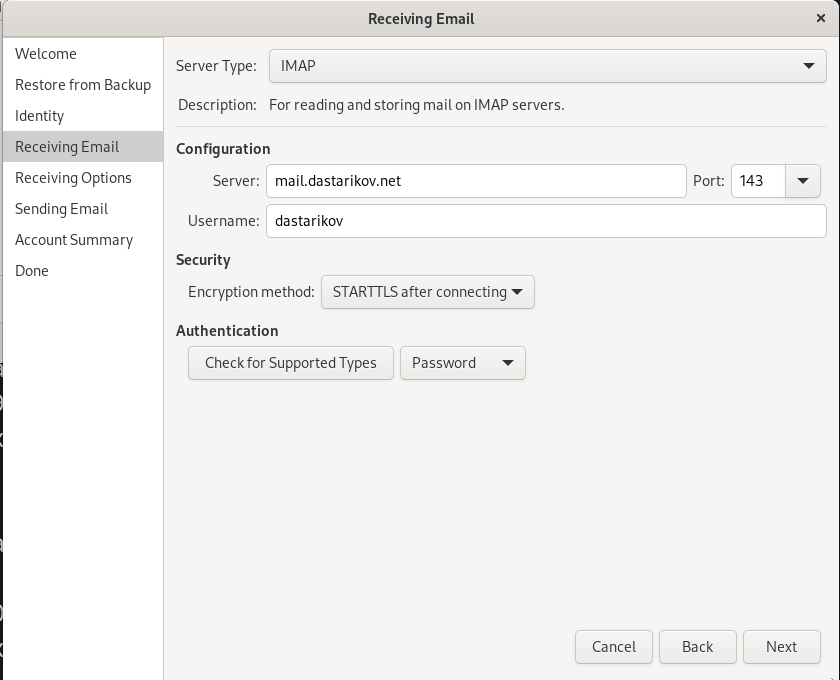
\includegraphics[width=\textwidth]{../images/image12.png}
    \captionof{figure}{Настройка входящих сообщений.}
    \label{12}
\end{center}
\begin{center}
    \centering
    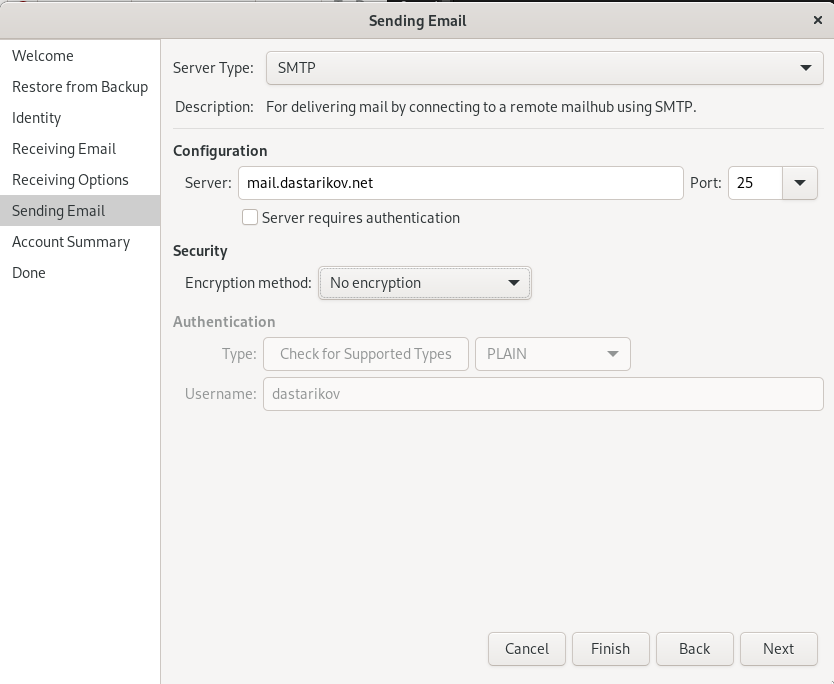
\includegraphics[width=\textwidth]{../images/image13.png}
    \captionof{figure}{Настройка исходящих сообщений.}
    \label{13}
\end{center}

\item Из почтового клиента отправили себе несколько тестовых писем и убедились, что они доставлены  (Рис. \ref{14} и \ref{15}).
\begin{center}
    \centering
    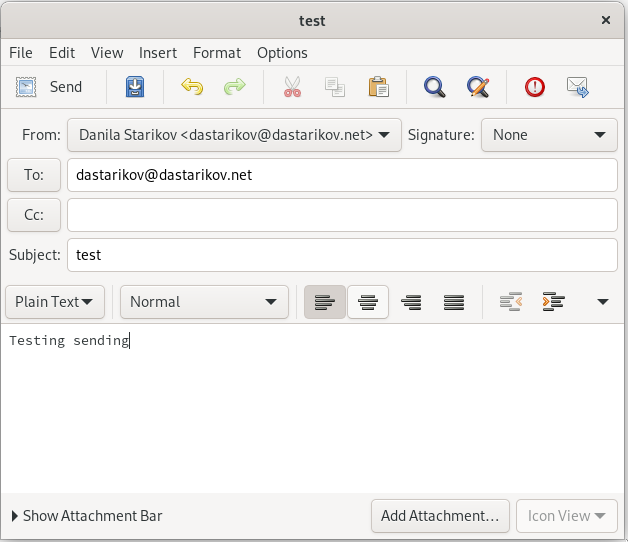
\includegraphics[width=\textwidth]{../images/image14.png}
    \captionof{figure}{Окно отправки письма.}
    \label{14}
\end{center}
\begin{center}
    \centering
    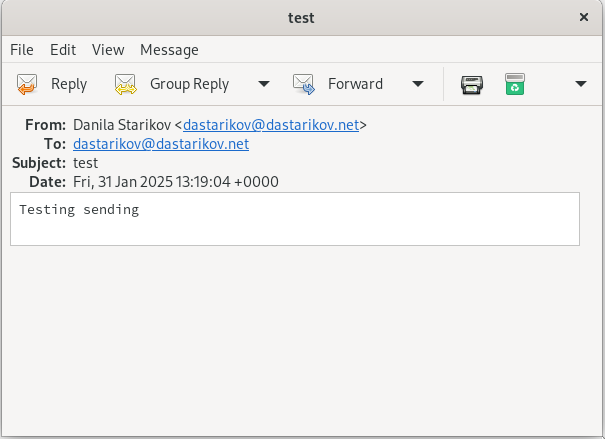
\includegraphics[width=\textwidth]{../images/image15.png}
    \captionof{figure}{Окна просмотра полученного письма.}
    \label{15}
\end{center}

\item Параллельно посмотрели, какие сообщения выдаются при мониторинге почтовой службы на сервере, а также при использовании \texttt{doveadm} и \texttt{mail} (Рис. \ref{17}-\ref{18}).
\begin{center}
    \centering
    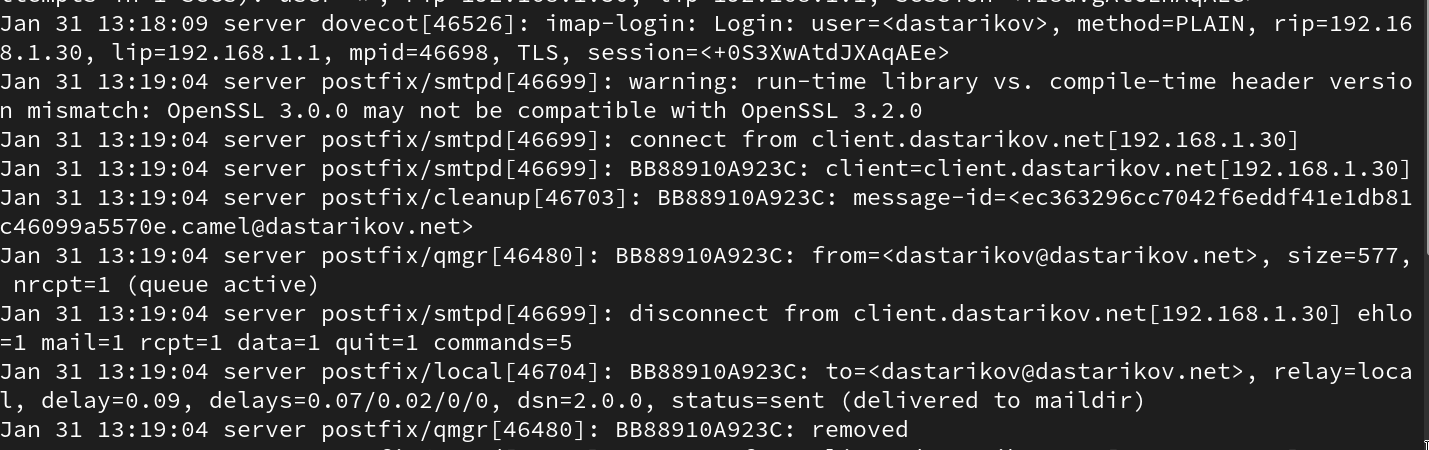
\includegraphics[width=\textwidth]{../images/image16.png}
    \captionof{figure}{Просмотр логов почтовой службы при отправке писем с клиента.}
    \label{16}
\begin{center}
    \centering
    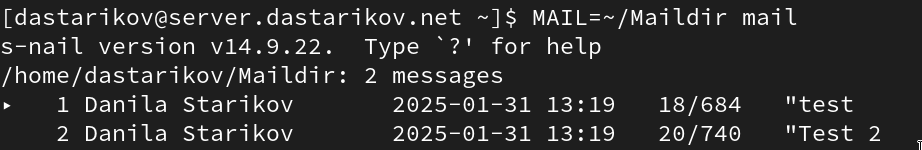
\includegraphics[width=\textwidth]{../images/image17.png}
    \captionof{figure}{Просмотр полученных писем через утилиту \texttt{mail}.}
    \label{17}
\end{center}
\begin{center}
    \centering
    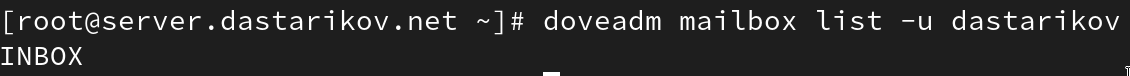
\includegraphics[width=\textwidth]{../images/image18.png}
    \captionof{figure}{Просмотр полученных писем через утилиту \texttt{doveadm}.}
    \label{18}
\end{center}

\end{center}

\item Проверили работу почтовой службы, используя на сервере протокол Telnet:
  \begin{itemize}
  \item подключились с помощью протокола Telnet к почтовому серверу по протоколу POP3 (через порт 110), ввели свой логин для подключения и пароль (Рис. \ref{19}):
    \begin{minted}{bash}
      telnet mail.dastarikov.net 110
      user dastarikov
      pass ******
    \end{minted}
\begin{center}
    \centering
    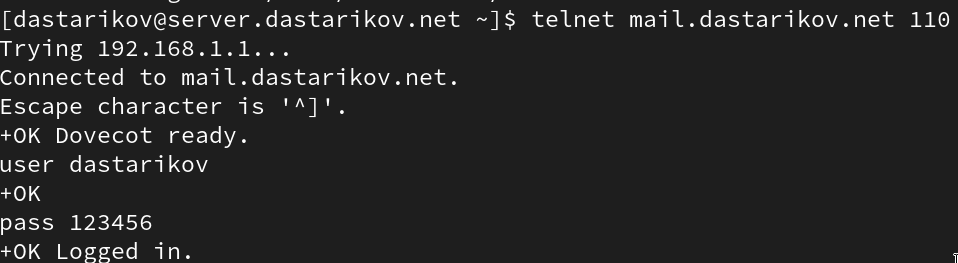
\includegraphics[width=\textwidth]{../images/image19.png}
    \captionof{figure}{Подключение к почтовому серверу через протокол Telnet.}
    \label{19}
\end{center}
  \item с помощью команды \texttt{list} получили список писем (Рис. \ref{20});
  \item с помощью команды \texttt{retr 1} получили первое письмо из списка (Рис. \ref{20});
  \item с помощью команды \texttt{dele 2} удалили второе письмо из списка (Рис. \ref{20});
  \item с помощью команды \texttt{quit} завершили сеанс работы с \texttt{telnet} (Рис. \ref{20}).
  \end{itemize}
\begin{center}
    \centering
    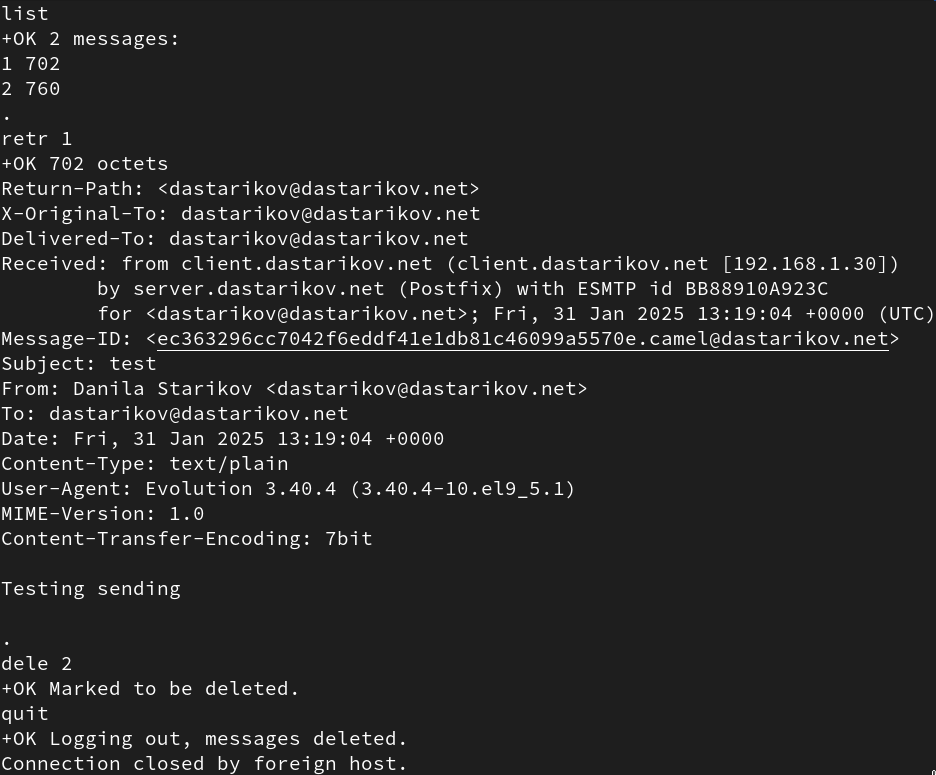
\includegraphics[width=\textwidth]{../images/image20.png}
    \captionof{figure}{Работа с почтовым сервером через telnet.}
    \label{20}
\end{center}

\end{enumerate}
\subsection{Внесение изменений в настройки внутреннего окружения виртуальной машины}
\begin{enumerate}

\item На виртуальной машине \texttt{server} перешли в каталог для внесения изменений в настройки внутреннего окружения \texttt{/vagrant/provision/server/}. В соответствующие подкаталоги поместили конфигурационные файлы Dovecot:
\begin{minted}{bash}
  cd /vagrant/provision/server
  mkdir -p /vagrant/provision/server/mail/etc/dovecot/conf.d
  cp -R /etc/dovecot/dovecot.conf /vagrant/provision/server/mail/etc/dovecot/
  cp -R /etc/dovecot/conf.d/10-auth.conf /vagrant/provision/server/mail/etc/dovecot/conf.d/
  cp -R /etc/dovecot/conf.d/auth-system.conf.ext /vagrant/provision/server/mail/etc/dovecot/conf.d/
  cp -R /etc/dovecot/conf.d/10-mail.conf /vagrant/provision/server/mail/etc/dovecot/conf.d/
\end{minted}
\item Внесли изменения в файл \texttt{/vagrant/provision/server/mail.sh}, добавив в него строки:
\begin{itemize}
  \item по установке Dovecot и Telnet;
  \item по настройке межсетевого экрана;
  \item по настройке Postfix в части задания месторасположения почтового ящика;
  \item по перезапуску Postfix и запуску Dovecot.
\end{itemize}
\begin{minted}{bash}
  #!/bin/bash
  echo "Provisioning script $0"
  echo "Install needed packages"
  dnf -y install postfix
  dnf -y install dovecot
  dnf -y install telnet
  echo "Copy configuration files"
  cp -R /vagrant/provision/server/mail/etc/* /etc
  chown -R root:root /etc/postfix
  restorecon -vR /etc
  echo "Configure firewall"
  firewall-cmd --add-service smtp --permanent
  firewall-cmd --add-service pop3 --permanent
  firewall-cmd --add-service pop3s --permanent
  firewall-cmd --add-service imap --permanent
  firewall-cmd --add-service imaps --permanent
  firewall-cmd --add-service smtp-submission --permanent
  firewall-cmd --reload
  echo "Start postfix service"
  systemctl enable postfix
  systemctl start postfix
  echo "Configure postfix"
  postconf -e 'mydomain = user.net'
  postconf -e 'myorigin = $mydomain'
  postconf -e 'inet_protocols = ipv4'
  postconf -e 'inet_interfaces = all'
  postconf -e 'mydestination = $myhostname, localhost.$mydomain, localhost, $mydomain'
  #postconf -e 'mynetworks = 127.0.0.0/8, 192.168.0.0/16'
  echo "Configure postfix for dovecot"
  postconf -e 'home_mailbox = Maildir/'
  echo "Configure postfix for auth"
  postconf -e 'smtpd_sasl_type = dovecot'
  postconf -e 'smtpd_sasl_path = private/auth'
  postconf -e 'smtpd_recipient_restrictions = reject_unknown_recipient_domain, permit_mynetworks, reject_non_fqdn_recipient, reject_unauth_destination, reject_unverified_recipient, permit'
  postconf -e 'mynetworks = 127.0.0.0/8'
  echo "Configure postfix for SMTP over TLS"
  cp /etc/pki/dovecot/certs/dovecot.pem /etc/pki/tls/certs
  cp /etc/pki/dovecot/private/dovecot.pem /etc/pki/tls/private
  postconf -e 'smtpd_tls_cert_file=/etc/pki/tls/certs/dovecot.pem'
  postconf -e 'smtpd_tls_key_file=/etc/pki/tls/private/dovecot.pem'
  postconf -e 'smtpd_tls_session_cache_database = btree:/var/lib/postfix/smtpd_scache'
  postconf -e 'smtpd_tls_security_level = may'
  postconf -e 'smtp_tls_security_level = may'
  postfix set-permissions
  restorecon -vR /etc
  systemctl stop postfix
  systemctl start postfix
  systemctl restart dovecot
\end{minted}
\item На виртуальной машине \texttt{client} в каталоге \texttt{/vagrant/provision/client} скорректировали файл \texttt{mail.sh}, прописав в нём:
\begin{minted}{bash}
  dnf -y install evolution
\end{minted}
\end{enumerate}

\section{Выводы}
В результате выполнения лабораторной работы приобрели практические навыки по установке и простейшему конфигурированию POP3/IMAP-сервера.
\end{document}
